\documentclass{beamer} 

% Michael Maier, 2013.
% CC-BY-SA

\usepackage[utf8]{inputenc}
\usepackage[ngerman]{babel}

\title{OpenStreetMap - Von Community, Open Data und effizientem Mappen} 
\author{Michael Maier \textless Michael.Maier@student.tugraz.at\textgreater} 
\date{21. Juni 2013} 

\usetheme{Antibes}

\hypersetup{colorlinks=true,urlcolor=blue,linkcolor=white}

\usepackage{xcolor}
\definecolor{olive}{rgb}{0.3, 0.4, .1}
\definecolor{fore}{RGB}{249,242,215}
\definecolor{back}{RGB}{51,51,51}
\definecolor{title}{RGB}{255,0,90}
\definecolor{dgreen}{rgb}{0.,0.6,0.}
\definecolor{gold}{rgb}{1.,0.84,0.}
\definecolor{JungleGreen}{cmyk}{0.99,0,0.52,0}
\definecolor{BlueGreen}{cmyk}{0.85,0,0.33,0}
\definecolor{RawSienna}{cmyk}{0,0.72,1,0.45}
\definecolor{Magenta}{cmyk}{0,1,0,0}

%\usebackgroundtemplatei{
%
\includegraphics[width=\paperwidth,
%height=0.8\paperheight]{mag_map.png}
%}

\begin{document}

%\maketitle

\begin{frame} 


\begin{figure}
  \centering
  
\includegraphics[width=.5\textwidth]{mag_map.png}
\end{figure}

\begin{center}
\Huge{OpenStreetMap\\}
\end{center}

\begin{center}
\Large{\emph{Von Community, Open Data und effizientem Mappen}}
\end{center}

\end{frame}



\begin{frame}{Vorstellung}

  \begin{itemize}
    \item Michael Maier \textless \href{mailto:Michael.Maier@student.tugraz.at}{Michael.Maier@student.tugraz.at}\textgreater
    \item Telematik-Student an der TU Graz 
    \item OpenStreetMap seit Juli 2010
    \item Leite den Grazer Stammtisch seit Mai 2011
    \item Vorträge, Workshops und Auftragsarbeiten rund um OpenStreetMap
	    \pause
    \begin{itemize}
      \item OSM-username: \emph{\href{http://www.openstreetmap.org/user/species}{species}}
      \item Bereich Graz, Leoben mit dem Fahrrad, Motorrad und Öffis
      \item Github-Account: \emph{\href{https://github.com/species}{species}}
      \item Twitter-Account: \emph{\href{https://twitter.com/osmgraz}{@osmgraz}}
    \end{itemize}
  \end{itemize}
\end{frame}

\section{Einleitung}

\begin{frame}{Inhalt}
	Plan für Heute:
	\vspace{7mm}
	\begin{itemize}
		  \item Community
			  \pause
			  \vspace{7mm}
		  \item Open Government Data
			  \pause
			  \vspace{7mm}
		  \item Effizientes Mappen
	  \end{itemize}
\end{frame}

\section{Community}

\begin{frame}{Community}
	OSM ist ein soziales Projekt!

	\begin{center}
	  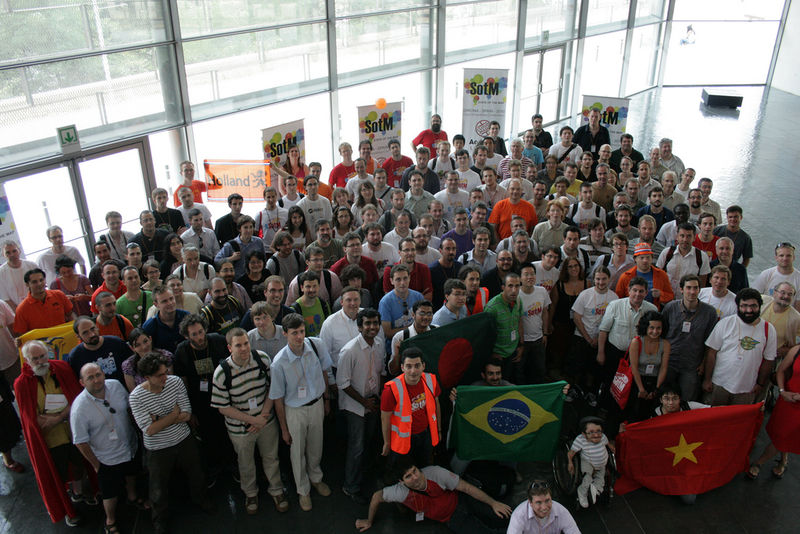
\includegraphics[width=5.5cm]{sotm.jpg}
	\end{center}

	\begin{itemize}
		  \item Eine Community wächst selten von alleine...
		  \item Motivation der Leute steigt beim gemeinsam arbeiten
		  \item Austausch steigert Effizienz
	  \end{itemize}
\end{frame}

\begin{frame}{Community aufbauen}
	Wie bringt man die Leut zamm?
	\pause

	\begin{columns}[c] % the "c" option specifies center vertical alignment
		    \column{.5\textwidth}
	\begin{itemize}
		\item Events!
\vspace{4mm}
		\begin{itemize}
			  \item Stammtische
				\vspace{3mm}
			  \item Mapping Parties
				  \vspace{3mm}
			  \item Hackathons
		\end{itemize}
	\end{itemize}
		\column{.5\textwidth}
	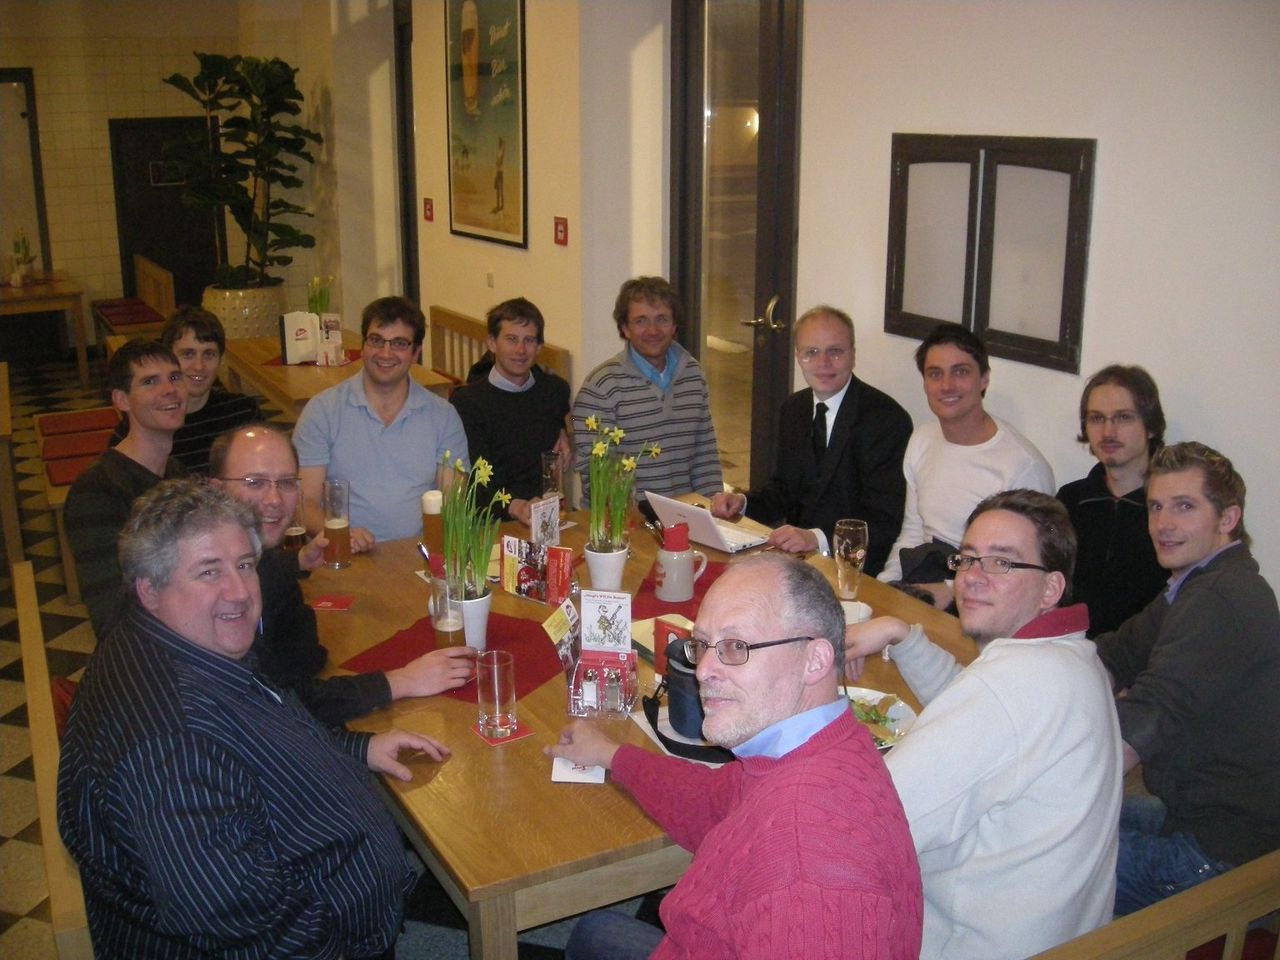
\includegraphics[width=5.5cm]{Salzburg_stammtisch.jpg}
\end{columns}

\end{frame}

\begin{frame}{Events organisieren}
	Checkliste für ein Event:
				  \vspace{3mm}
	\begin{itemize}
		\item Thema? Sich kennenlernen, Erfahrungsaustausch!
		\item Ort? Ruhiges Lokal mit gutem Essen, Nichtraucher, Barrierefrei, mit Öffis erreichbar
		\item Termin? Anfangs Doodle, später regelmäßig
		\item Teilnehmer finden? Wo ankündigen?
	\end{itemize}
\end{frame}

\begin{frame}{Event ankündigen:}
	Eventankündigung wo:
	\begin{itemize}
		\item Mailingliste \href{http://lists.openstreetmap.org/listinfo/talk-at}{talk-at}
		\item OSM-wiki Startseite: \href{http://wiki.openstreetmap.org/wiki/Current\_events}{Current Events}
		\item Social Media: Twitter, FB, webtermine.at
		\item schauen, dass man auf \href{http://blog.openstreetmap.de/}{OSM-Blog} erwähnt wird...
		\item Newsgroups, Foren, Geo-Newsletter?
		\item im Wiki Community-Seite anlegen, dann erscheints auf \href{http://openstreetmap.de}{openstreetmap.de}
		\item persönliche Emails, OSM-PMs
		\begin{itemize}
			\item  Arbeit, aber lohnt: Neue User persönlich einladen - RSS-Feed von \$Region abonnieren!
		\end{itemize}
	\end{itemize}
\end{frame}

\begin{frame}{Sich selbst sozialisieren}
	
	\begin{itemize}
		\item Mailinglisten lesen
		\begin{itemize}
			\item wers mag: es gibt auch ein \href{http://forum.openstreetmap.org/viewforum.php?id=14}{Forum}...
		\end{itemize}
		\item Persönlicher "Blog": OSM Diary - Auf gute Beiträge kommen Rückmeldungen!
		\item Im Wiki bzw. auf seiner OSM-Profilseite Kurzabriss über sich selbst und seine Projekte reingeben
		\item Eigene Projekte auf \href{http://github.com}{Github} stellen! Github ist eins der größten sozialen Netzwerke weltweit!
		\item Aktiv im Wiki mitarbeiten: bei Proposals mitvoten oder selbst erstellen, Seiten seiner Region mitgestalten
	\end{itemize}
\end{frame}

\subsection{Public Relations}

\begin{frame}{OSM promoten}
	
	\begin{itemize}
		\item Bei Mappingparties Medienwirksamkeit erzeugen
		\item OGD-Stammtische
		\item Open-Source-Events (*Linuxtage), BarCamps
		\item Blogs zu GIS/Open Data, zB opendatagraz.at
		\item Geo-Konferenzen, Bürgerbeteiligungsinitiativen
			\pause
		\item immer ein paar Folder/Visitenkarten dabeihaben
	\end{itemize}
	\begin{center}
		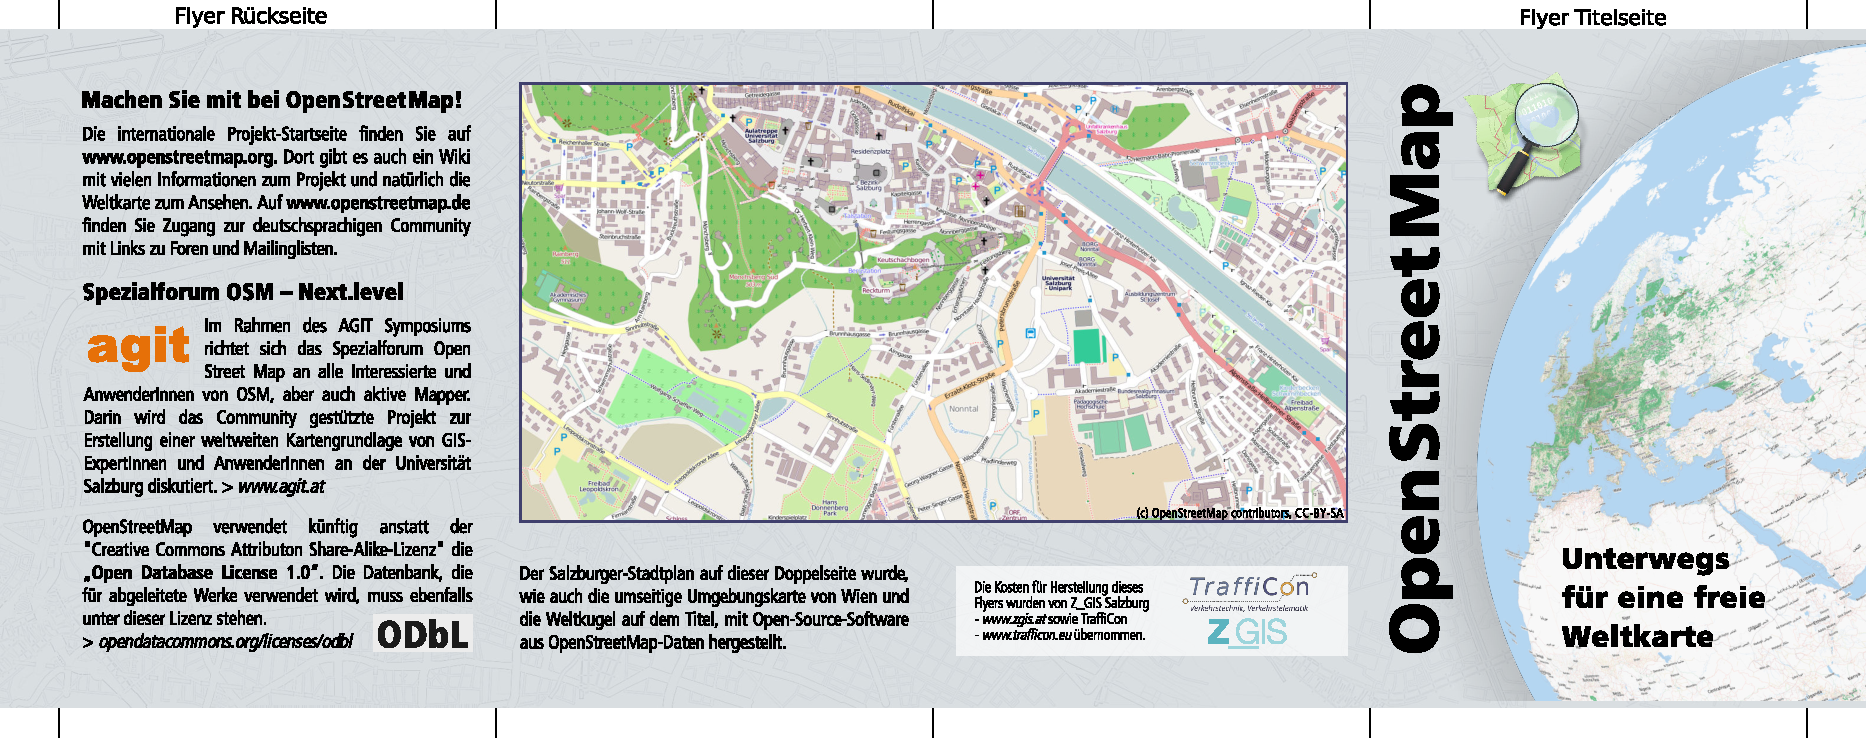
\includegraphics[width=8.5cm]{Osmflyer-front-aut.pdf}
	\end{center}
\end{frame}

\begin{frame}{Messen/Events}
	Checkliste für einen Messestand:
	\begin{itemize}
		\item großes Banner sowie Karten aufhängen
		\item Flyer, Sticker auflegen
		\item Fanartikel: Warnwesten, Tassen, Pins
		\item Großen Bildschirm mit Eye-Catcher, z.B. \href{http://osmlab.github.io/show-me-the-way/}{Live-Edits}
	\end{itemize}
	\begin{columns}[t] % the "c" option specifies center vertical alignment
		\begin{column}[T]{.4\textwidth}

	\begin{itemize}
		\item Editierstation(en)
		\item Garmin-Tankstelle
		\item mindestens zu zweit sein
	\end{itemize}
	\end{column}

	\begin{column}[T]{.5\textwidth}
				    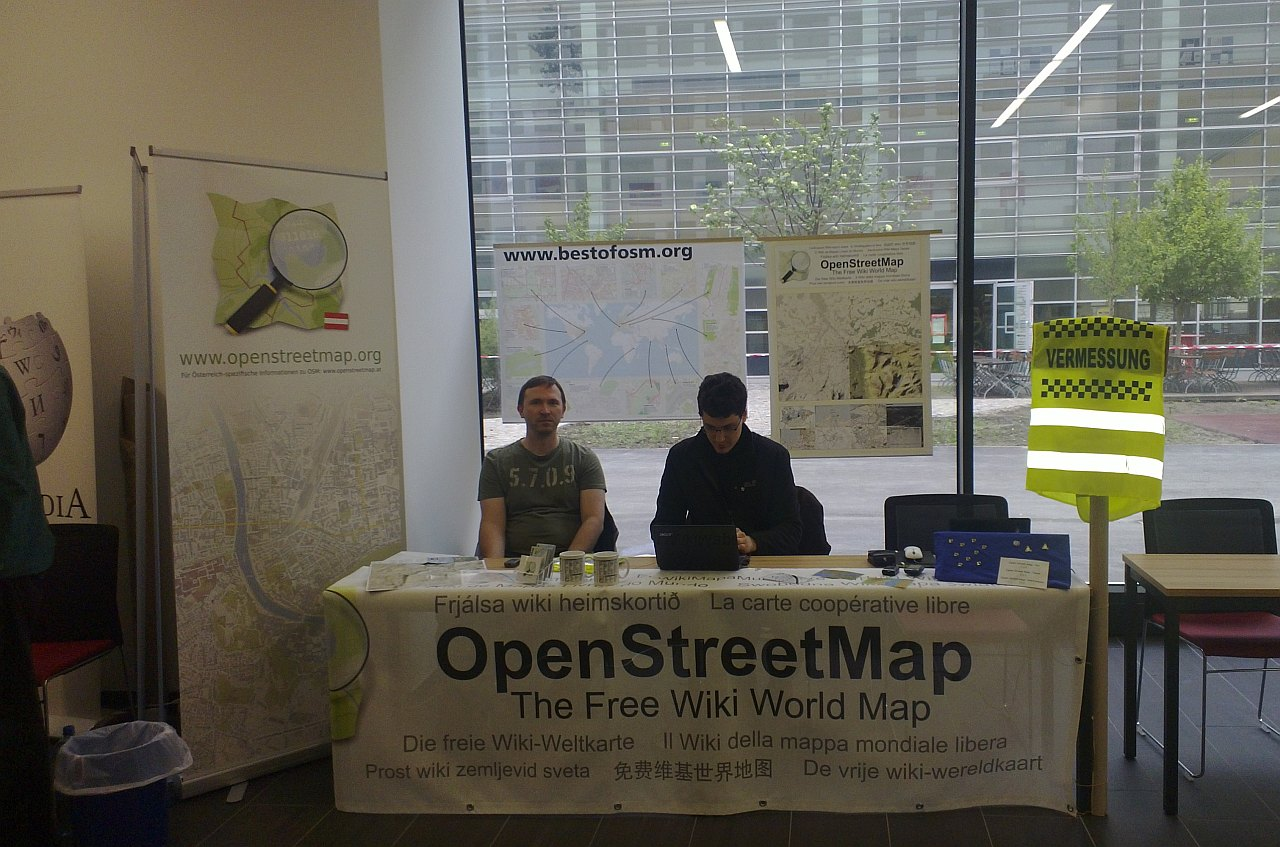
\includegraphics[width=4.5cm]{liwo2013_stand_big.jpg}
				    \end{column}
				    \end{columns}
\end{frame}

\subsection{\#switch2osm}

\begin{frame}{OSM erklären}
	So simpel wie möglich...
	\begin{itemize}
		\item Fahrradnavi! Rollstuhlkarte! Nichtraucherkarte!
		\item Hochaktuell
		\item Ich kann Fehler selbst korrigieren
		\item Roh-Daten sind frei
		\item darf es offline nutzen - z.B. im Ausland
		\item "Wikipedia für Karten"
	\end{itemize}
	
\end{frame}

\begin{frame}{Kritik}
	Ja, aber es darf ja jeder alles ändern?
	\vspace{5mm}
	\begin{columns}[c]
		\begin{column}[T]{.4\textwidth}
			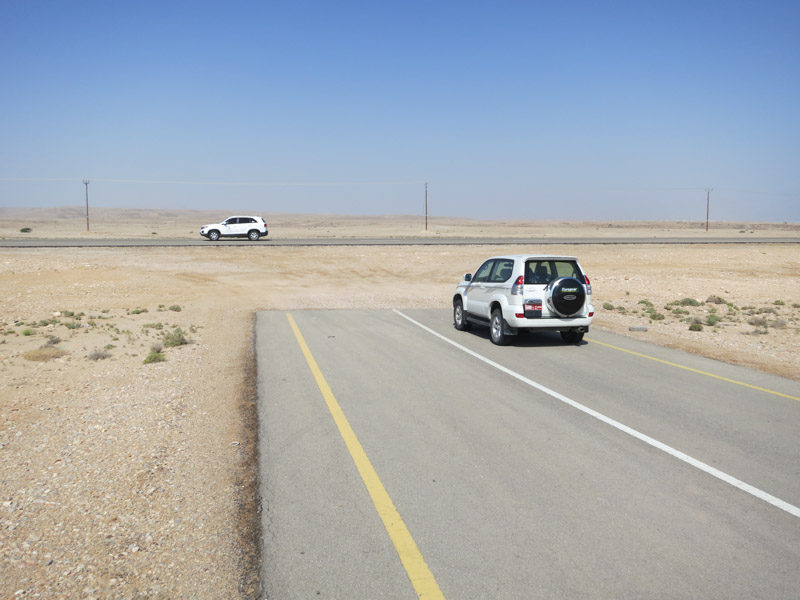
\includegraphics[width=4.5cm]{unconnected.jpg} \\
			{\TINY CC-BY \url{http://www.bodenseepeter.de}}
		\end{column}
		\pause
		\begin{column}[T]{.6\textwidth}
			\begin{itemize}
				\item Es gibt in OSM nur "Ground Truth", keine verschiedenen Meinungen über Politiker 
				\item Eintrittsschwelle ist im ggs zur Wikipedia höher (keine Anonymous edits)
				\item Erfahrene Mapper kontrollieren ihr Gebiet mittels RSS-Feed
			\end{itemize}
		\end{column}
	\end{columns}
\end{frame}

\begin{frame}{Für Geographen}
	Die meisten Geo-Menschen kennen OSM noch nicht oder sind skeptisch...
	\pause
	\vspace{5mm}
	Wie ist die Geo-Welt derzeit?
	\pause
	\begin{itemize}
		\item Viele Organisationen haben Daten in unterschiedlichen Formaten:
			\begin{itemize}
				\item Projektionen - der Graus eines jeden Geo-Studenten!
				\item inkompatible Dateiformate und Datenbanken
				\item Konvertierung nur Lossy möglich
			\end{itemize}
		\item in unterschiedlichen Lizenzen, wenn frei dann nur nichtkommerziell nutzbar - nicht "Open"
		\item zu zu hohen Preisen, wenn ich Daten kommerziell Nutzen will
	\end{itemize}
\end{frame}

\begin{frame}{Jemand braucht Daten...}
	Wenn ich für irgendwas Daten brauche:
	\vspace{5mm}
	Wer hat Daten?
	
	\begin{itemize}
		\item Teleatlas, Navteq - wird sicher teuer...
			\pause
		\item Offizielle Stellen anfragen...
			\begin{itemize}
				\item Wenn sie denn eine Webseite haben?
				\item anrufen...
				\item Bürozeiten, Urlaub?
			\end{itemize}
	\end{itemize}
	Ich warte lange Amtswege ab und zahle womöglich utopische Preise für veraltetes Kartenmaterial
\end{frame}

\begin{frame}{Unterschiedliche Quellen...}
	Wenn ich Daten nicht nur von einer Stelle brauche, muß ich sie mergen...
	\begin{columns}[c]
		                \begin{column}[T]{.7\textwidth}
	\begin{itemize}
		\item An verschiedenen Stellen anfragen
			\begin{itemize}
				\item Adressen vom BEV 
				\item Einwohnerzahlen von der Statistik Austria
				\item Landnutzungen vom Forstamt
				\item ÖPNV-Daten vom Verkehrsverbund
				\item ...
			\end{itemize}
			\pause
		\item Projektionen anpassen
		\item Gebietsweise Überschneidungen?
		\item Attributbezeichnungen mergen
	\end{itemize}
\end{column}
\begin{column}[T]{.3\textwidth}

	
\includegraphics[width=2cm]{gis-stmkl.png} 
	\vspace{4mm}

	
\includegraphics[width=2cm]{bev.png} 
	\vspace{4mm}

	
\includegraphics[width=2cm]{gis-ktn.png} 
	\vspace{4mm}

	
\includegraphics[width=2cm]{ktn-linien.png} 

\end{column}
\end{columns}

\end{frame}

\begin{frame}{Der Traum...}
	Sollte es nicht so sein:
	\begin{itemize}
		\item Es gibt weltweit EIN Portal für ALLE Geodaten
		\item In weltweit einheitlichem Format (WGS84, Dezimalgrad)
		\item Wo ich nicht warten muß, sondern einfach einen Ausschnitt wählen kann und runterladen
		\item Alle Daten unter einen offenen Lizenz nutzen kann
	\end{itemize}

	\begin{columns}[c] % the "c" option specifies center vertical alignment
		    \column{.5\textwidth}
		    \begin{center}
	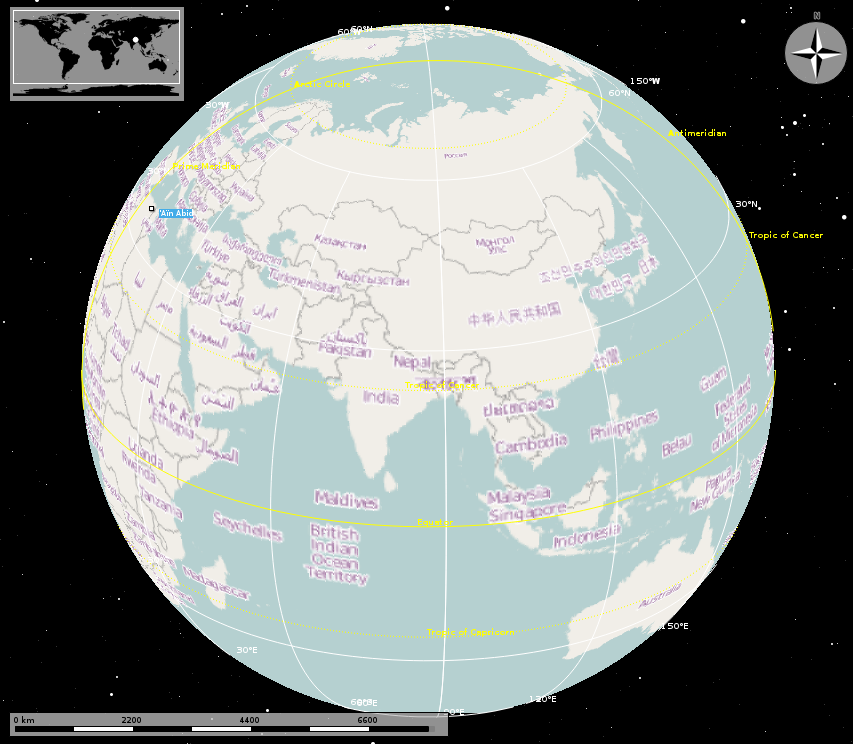
\includegraphics[width=3.5cm]{marble.png}
	\end{center}
		    \column{.5\textwidth}
	    \begin{center}
		
\includegraphics[width=1.5cm]{cc-by-sa.png}
	\end{center}
\end{columns}

\end{frame}

\section{Open Government Data}

\begin{frame}{Motivation}
	Sollten Daten, die mit Steuergeld erfasst werden, nicht öffentlich zugänglich sein?

	\vspace{3mm}
	Beispiel BEV:
	\begin{itemize}
		\item Gemeinden sind verpflichtet, Adressen dem BEV zu melden und zu verorten
		\item BEV verkauft diese Adressen
		\item Gemeinden verlieren jedes Nutzungsrecht an den Adressen
		\item z.B. das Land Steiermark muss für die Adressen wiederum ans BEV zahlen
			\pause
		\begin{itemize}
			\item und eine Zusatzgebühr, um sie im WebGIS-anzeigen dürfen
		\end{itemize}
	\end{itemize}

	 Und das mit unseren Steuergeldern ... macht doch Magenweh, oder?

	 \vspace{3mm}
	 Beispiel USA: GIS-Daten (TIGER) dort schon lange Public Domain!
\end{frame}

\begin{frame}{Open Data}
	\begin{block}{Open Data Definition} 
	“A piece of data or content is open if anyone is free to use, reuse, and redistribute it — subject only, at most, to the requirement to attribute and/or share-alike.”
\end{block}


Ich darf... \hfill \url{http://opendefinition.org/}
	\begin{itemize}
		\item verwenden
		\item verändern
		\item weiterverbreiten
	\end{itemize}
	
	Maximal CC-BY oder CC-BY-SA

	\pause
	\vspace{3mm}
AT: CC-BY 3.0 at
\begin{itemize}
		                \item nur die Datenquelle muss genannt werden
			\end{itemize}
\end{frame}

\begin{frame}{OpenStreetMap-Lizenz}

Die Daten stehen unter der Open Database License - Entspricht etwa Creative Commons - Attribution - Sharealike für Daten.
\begin{itemize}
  \item Jeder darf die Daten, auch kommerziell verwenden
  \item Quelle: ``OpenStreetMap and Contributors, ODbL'' muß angegeben werden.
\end{itemize}

 \begin{center}
 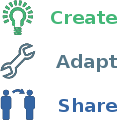
\includegraphics[width=1cm]{ODbL.png}
 \hspace{2cm}
 
\includegraphics[width=1.5cm]{cc-by-sa.png}
 \end{center}

\pause
Die Web-karten (gerenderten Tiles) auf \href{http://osm.org}{openstreetmap.org} sind CC-BY-SA, beachte \href{http://wiki.openstreetmap.org/wiki/Tile\_usage\_policy}{Tile Usage Policy}!

\end{frame}


\begin{frame}{OGD in Österreich}
	Metaportal: \url{http://data.gv.at}

	\vspace{3mm}

	Derzeitige veröffentlichende Stellen:
	\begin{itemize}
		\item Wien
		\item Linz
		\item Engerwitzdorf
		\item Graz
		\item Land Steiermark
			\pause
		\item Land Kärnten (Beta)
	\end{itemize}
\end{frame}

\begin{frame}{Land Kärnten}
	
	\href{http://www.kagis.ktn.gv.at/278870\_DE-GEODATEN-OGD-Kaernten\_(beta)}{kagis.ktn.gv.at/278870\_DE-GEODATEN-OGD-Kaernten\_(beta)}
	\begin{itemize}
		\item Höherrangiges Straßennetz (gml)
		\item Übergeordnetes Radwegenetz (Shape)
		\item Haltestellen (Shape)
		\item Buslinien (Shape)
		\item Park- and Ride Anlagen (Shape)
		\item Sportstätten (Shape)
		\item Schutzgebiete (Natur etc.) (gml)
	\end{itemize}
	\vspace{3mm}
	CC-BY 3.0 AT "Land Kärnten - data.ktn.gv.at" \hfill 
\includegraphics[width=2cm]{cc-by.png}
\end{frame}

\begin{frame}{Updates aus OGD?}
	Derzeit von offizieller Seite kaum bedacht...
	\pause

	\vspace{3mm}
	Meist nur die letzte Version online :-/

	\pause
	\vspace{3mm}
	Wir brauchen Diffs...

	\pause
	\vspace{3mm}
	Versionierung heißt das Zauberwort!

	\begin{columns}[c] 
	    \column{.5\textwidth}
		\begin{center}
			{\LARGE $\rightarrow$ Github}
		\end{center}
	    \column{.5\textwidth}
		\begin{center}
			
\includegraphics[width=2cm]{github.jpg}
		\end{center}
	\end{columns}

	\vspace{3mm}
	z.B. \url{https://github.com/species/OGD-ktn-daten}

\end{frame}

\subsection{Arbeiten mit OGD}

\begin{frame}{OGD in OSM}
	Wie kann ich OGD in OSM verwenden?

	\begin{columns}[c] 
	    \column{.5\textwidth}
		\begin{center}
			
\includegraphics[width=2cm]{josm-latest.png}
		\end{center}
	    \column{.5\textwidth}
		\begin{center}
			
\includegraphics[width=2cm]{qgis-icon.png}
		\end{center}
	\end{columns}


	\begin{itemize}
		\item Shape: in JOSM öffnen!
		\pause
		\begin{itemize}
			\item benenne Spalten nach OSM-Standards um
			\item lösche Überflüssiges
		\end{itemize}
		\item füge source="Land Kärnten - data.ktn.gv.at" hinzu
		\item Merge mit OSM-Daten
		\item upload :-)
	\end{itemize}
	\pause
	\hfill ... soweit die Theorie

\end{frame}

\begin{frame}{OGD-Praxis in OSM}
	QGIS fast immer nötig... \pause \\
	\hfill \textcolor{red}{Vorsicht: OSM-Plugin noch nicht 64bit-kompatibel!}
\pause
	\begin{itemize}
		\item für JOSM muss Shape in WGS84 sein $\rightarrow$ bei Bedarf umprojizieren!
		\item alles andere (gml,csv,...) muss in Shape konvertiert werden
		\item Mergen großer Datensätze mit OSM mit QGIS viel einfacher:
		\begin{itemize}
			\item Lade vorhandene Daten aus OSM und neue
			\item filtere Doppelte mittels Bufferzonen 
			\item 'Neue' könnten oft 1:1 importiert werden
			\item Doppelte meist von Hand mergen :-/
		\end{itemize}
		\item Speichern als Shape, öffnen mit JOSM, tags fixen
	\end{itemize}
\end{frame}
\subsection{GIS $\iff$ OSM}

\begin{frame}{Shape-Konvertieren}

Shapefile vs. OSM-XML
\vspace{3mm}

 \begin{columns}[c]
            \column{.5\textwidth}
	OSM-XML
		\begin{itemize}
			\item XML, ev. gezippt, oder dbf
			\item Immer WGS84, Dezimalgrad
			\item UTF-8
			\item key-value pairs, Freitext
			\item Beliebige Anzahl Attribute
			\item Node, Way, Relation (+Meta-Rels)
		\end{itemize}
            \column{.5\textwidth}
	Shapefile
		\begin{itemize}
			\item 3+ verschiedene Dateien
			\item Beliebige Projektion
			\item Zeichensatz oft undefiniert
			\item max. 13 Zeichen/Spalte
			\item Fixe Spalten
			\item Punkte, Linien, Polygone (MPs)
		\end{itemize}
\end{columns}

\end{frame}

\begin{frame}{Shape 2 OSM}

	Das ist die leichte Übung...
	\vspace{3mm}

	JOSM mit opendata-Plugin kann Shapes lesen

	\begin{itemize}
		\item Shape öffnen
		\item als .osm.xml abspeichern
		\item muss als WGS84 vorliegen
	\end{itemize}
	Beachte Spaltennamen!
\end{frame}

\begin{frame}{OSM 2 Shape}
	Nicht ganz so einfach, 2 Möglichkeiten:
\vspace{3mm}

 \begin{columns}[c]
            \column{.5\textwidth}
	via PostgreSQL/PostGIS
		\begin{itemize}
			\item Benötigt PostgreSQL/PostGIS-Server
			\item DB-Import mittels osm2pgsql
			\item mit QGIS auf die DB connecten
			\item Speichern als Shape
		\end{itemize}
            \column{.5\textwidth}
	via .geojson
		\begin{itemize}
			\item QGIS kann nur 1 Datentyp!
			\item Aufsplitten nach Punkt, Linie, Polygon in JOSM
			\item als .geojson speichern
			\item in QGIS öffnen
			\item Speichern als Shape
		\end{itemize}
\end{columns}

\end{frame}

\section{Wie funktioniert OpenStreetMap?}

\begin{frame}{Technischer Hintergrund}

Es gibt eine zentrale Datenbank (PostgreSQL/PostGIS) für Schreibzugriffe (in GB).\\
\pause
Diese wird weltweit gespiegelt für Lesezugriffe mit unterschiedlichen Methoden:

\begin{itemize}
  \item API-Lesezugriffe werden über mehrere Spiegel-Server lastverteilt
  \item Rendering-Server nutzen eine lokale, minütlich aktualisierte Datenbank
  \item Extrakte zum Download siehe \href{http://wiki.osm.org/Planet}{wiki.osm.org/Planet}
  \item Für räumliche SQL-Abfragen: Overpass API, zB alle italienischen Restaurants in Graz
\end{itemize}

\end{frame}


\begin{frame}{Datenmodell}

Wurde von Informatikern ohne Geo-Vorbelastung erstellt:
\begin{itemize}
  \item Punkte (Koordinaten), $\Rightarrow$ ``Node'' 
\includegraphics[width=0.5cm]{node.png}
	\begin{itemize}
          \item POIs
\pause
\item Teile von Wegen
\end{itemize}
  \item Linienzüge sind eine Reihe von Nodes, $\Rightarrow$ ``Way'' 
\includegraphics[width=0.5cm]{way.png}
	\begin{itemize}
	  \item Wege, Flüsse, Hecken etc.
	\item können geschlossen sein: Gebäude, Flächen
\end{itemize}
\pause
  \item Gruppierungen von Ways/Nodes $\Rightarrow$ ``Relations'' 
\includegraphics[width=0.5cm]{relation.png}
	\begin{itemize}
          \item Streckenrelationen, zB ÖPNV-Routen, Radrouten
	\item Multipolygone (Zusammengesetzte Flächen mit Ausschnitten)
	\item Abbiegebeschränkungen (Way:von, Way:nach, Node:über)
	\item Meta-Relationen, zB für Verkehrsverbünde
	\end{itemize}
\end{itemize}

\end{frame}

\begin{frame}{Datenmodell 2}

Jedes Element kann Eigenschaften $\Rightarrow$ ``Tags'' haben, zB:
\begin{itemize}
  \item amenity = cafe 
\includegraphics[width=0.5cm]{cafe.png}
  \item highway = footway 
\includegraphics[width=1cm]{footway.png}
  \item building = yes  
\includegraphics[width=0.5cm]{building.png}
  \item landuse = farmland
\end{itemize}

Tags sind Freitext, beliebige Anzahl!

Standards werden im Wiki festgelegt, siehe \href{http://wiki.openstreetmap.org/wiki/DE:How\_to\_map\_a}{wiki/DE:How\_to\_map\_a}

\vspace{4mm}
\pause
\begin{itemize}
  \item Koordinaten sind in Dezimalgrad, WGS84. 
	\begin{itemize}
  \item 3D-Information werden als Tags eingetragen, zb ele=435
\end{itemize}
  \item Genauigkeit 7 Stellen, entspricht 1\,cm am Äquator.
  \item Standard-Dateiformat: XML
\end{itemize}

\end{frame}


\begin{frame}{3D ist die Zukunft!}
  3D-OSM Beispielkarte siehe \href{http://maps.osm2world.org/?zoom=17&lat=47.06156&lon=15.46983&layers=BF0FTFFF}{maps.osm2world.org}.

  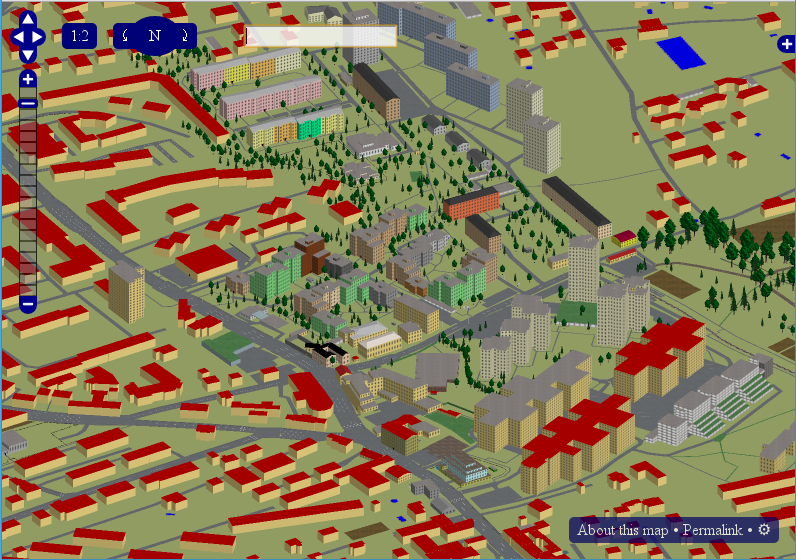
\includegraphics[width=0.9\textwidth]{3d.png}

\end{frame}

\begin{frame}{Hilfe}

\begin{itemize}
  \item Erste Station sollte das Wiki sein: \href{http://wiki.openstreetmap.org}{wiki.openstreetmap.org}
  \item Immer noch etwas unklar? $\Rightarrow$ Mailingliste \href{http://lists.openstreetmap.org/listinfo/talk-at}{talk-at}
  \pause
  \item Der nächste Stammtisch: \href{http://wiki.openstreetmap.org/wiki/Graz/Stammtisch}{Graz} monatlich - wieder am Mittwoch, 17.7.2013, im Rahmen der Open Week Graz im "Brot \& Spiele" Graz.
\end{itemize}

\end{frame}

\section{Ende}

\begin{frame}{Vielen Dank für die Aufmerksamkeit!}

  OSM-Folien am 21.6.2013, FH Kärnten, Villach
\vspace{1cm}

Folien unter: 
\includegraphics[width=1cm]{cc-by-sa.png}.
\vspace{1cm}

Erstellt mittels \LaTeX Beamer, Quelltext: \href{https://github.com/species/vortrag-osm-fh\_ktn\_6-2013}{Github}.
\vspace{1cm}

\href{mailto:michael.maier@student.tugraz.at}{Michael Maier}

Twitter: \href{https://twitter.com/osmgraz}{@osmgraz}
\end{frame}

\end{document}
